\documentclass[titlepage]{article}

\usepackage{tipa}
\usepackage{titlepic}
\usepackage{graphicx}
\usepackage{hyperref}
\usepackage{xcolor}
\usepackage{float}
\usepackage[export]{adjustbox}

\DeclareGraphicsExtensions{.pdf,.png,.jpg}

\definecolor{linkcol}{RGB}{50,50,50}
\hypersetup{
    colorlinks=true,
    linkcolor=linkcol
}


\title{
\includegraphics[width=200pt, height=260pt]{../../images/trdrop_logo_text.eps} \\[50pt]
Teardrop - a video analysis software}
\author{Alexander Isenko}
\date{}

\begin{document}

\maketitle

\newpage

\section{Description}

\textbf{trdrop} - pronounced [\textit{\textipa{'te@(r),drAp}}], is a marvelous video analysis software. It can calculate the frame rate of a raw input video, show frame tears, visualize the result and export it into a youtube friendly format. \\[2mm]
\hfill
\textbf{trdrop\_lib} is the core library which provides an interface to create a command line and a GUI interface for the provided functionality. \\[2mm]
\hfill
\textbf{trdrop\_cbin} is the command line interface which will be configurable through a config file and/or flags. The output can be streamed while being processed from VLC to get a preview.

\section{Formal description}

This project covers several themes of C++, mainly defined under the umbrella term \textit{offline feature extraction of big raw video data}. The task consists of creating a streaming interface to being able to process multiple GB sized videos, apply the feature detection and encode everything into a single video in constant space complexitiy.

\subsection{Functionality}

The following features are to be included in \textbf{v0.1}:

\begin{itemize}
    \item determine the real fps of the incoming video files
    \item show the fps as text in the video
    \item import up to 4 \texttt{.raw} video files with a size greater than 150 \texttt{GB}
    \item export the resulting video into a youtube friendly format (\href{https://support.google.com/youtube/answer/1722171}{google-terms})
    \item the resulting video can be streamed using VLC while it's being created
\end{itemize}

\subsection{Program Diagram}

\begin{figure}[H]
\hspace{-30mm}
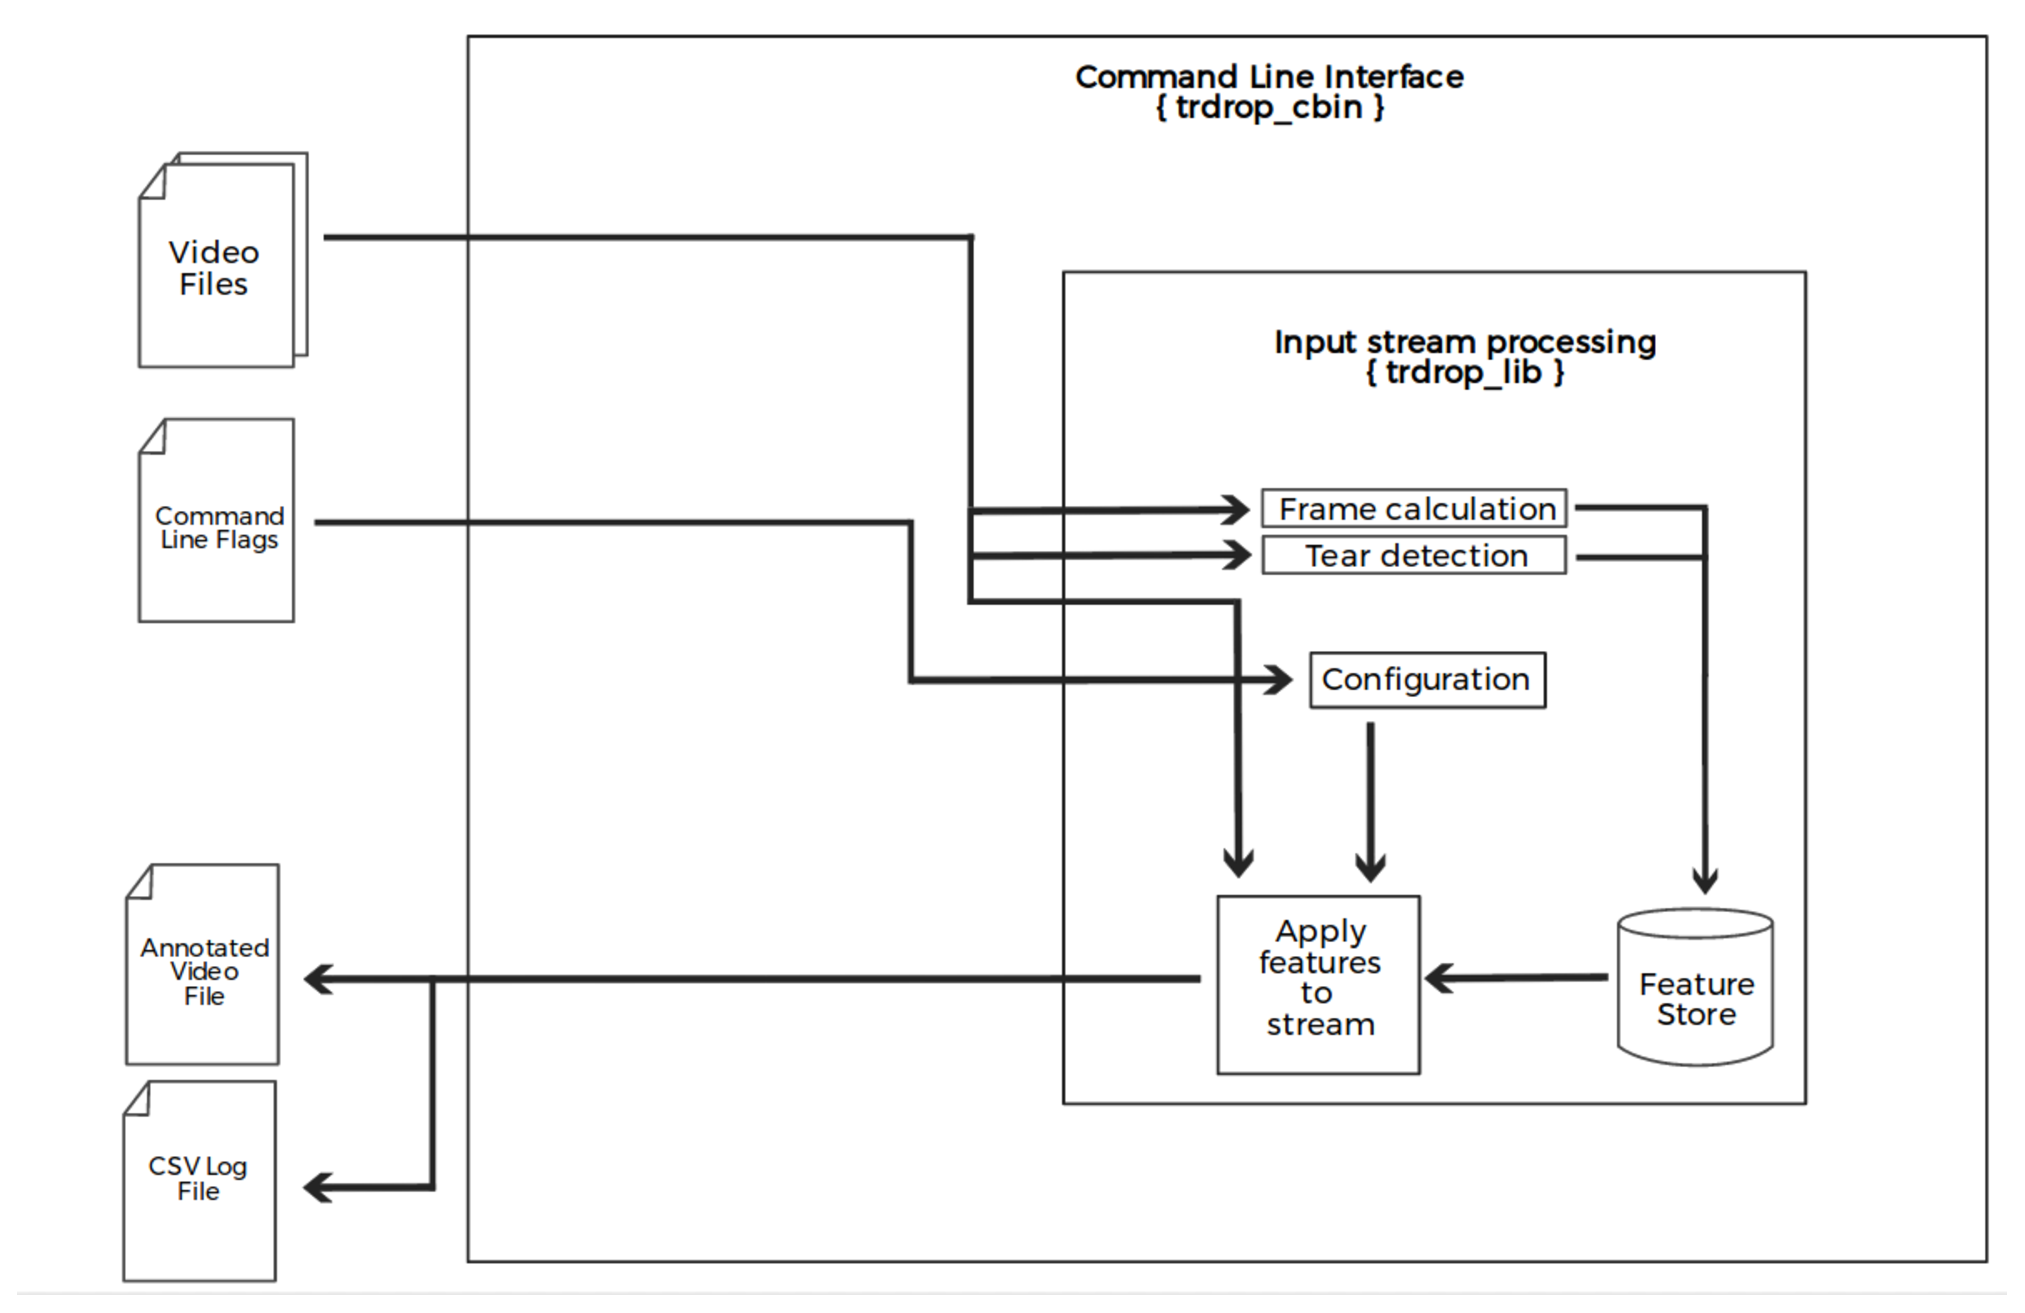
\includegraphics[width=500pt,left]{../../images/trdrop_diagram.eps}
\end{figure}

\section{Example usage}

\subsection{Command Line Interface}

\begin{verbatim}
# Creates a new annotated video with defaults
#
$ trdrop_cbin video_01.raw > converted_video.mp4

# Creates a new annotated video and VLC is used to visualize the result
#
$ trdrop_cbin video_01.raw > converted_video.mp4 | vlc

# Creates a new annotated video from multiple inputs
#
$ trdrop_cbin video_01.raw video_02.raw video_03.raw video_04.raw > converted_video.mp4
\end{verbatim}


\section{Future work}

\end{document}

